\chapter{Results and Evaluation}

This chapter compare the results obtained in each stage and how those results are supported to narrow down the research to find number of optimal thread pool for given program. In the early phases broader measurements metrics ( average latency, throughput, slandered divination of latency and throughput, 99th percentile of latency, error rate ) were analyzed to compare  architectures. In the later phases average latency (in milliseconds) is used as main metric to compare performance. Chapter 3 explains the these metrics in detail.

In the first phase following architectures were implemented,

\begin{itemize}
	\item Ballerina existing architecture
	\item Removing Ballerina Scheduler
	\item Blocking thread pool in Netty Layer (Netty \acrshort{OIO}) 
\end{itemize}

\section{Results comparison of different architectures}

\begin{figure}[htbp]
	\begin{center}
		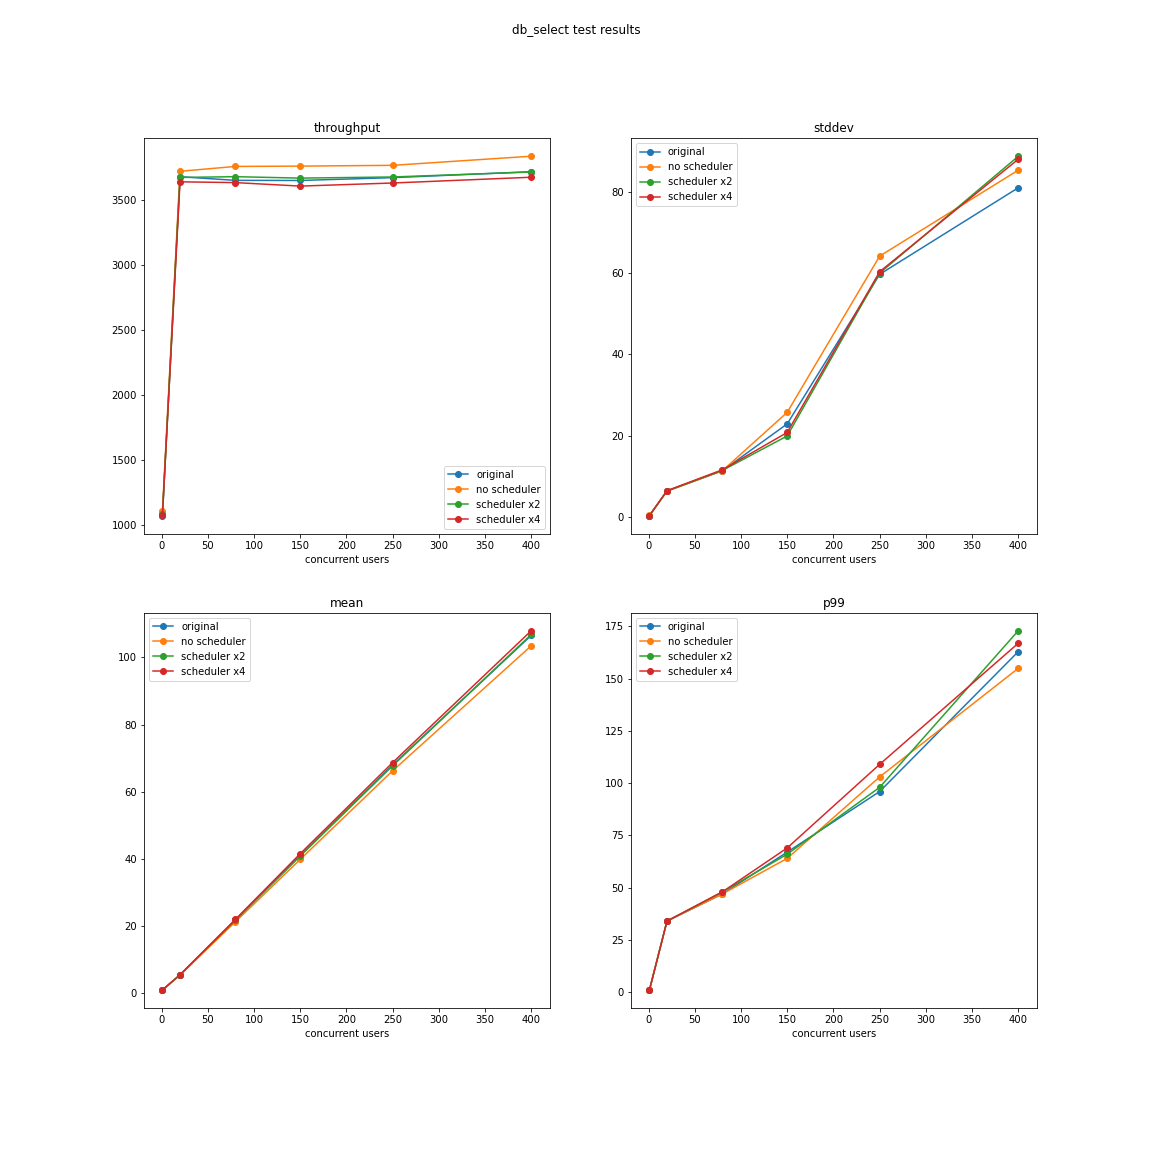
\includegraphics[scale=0.3]{figures/db_select test results.png}
	\end{center}
	\caption{Database select results}
	\label{db_select_results}
\end{figure}

\begin{figure}[htbp]
	\begin{center}
		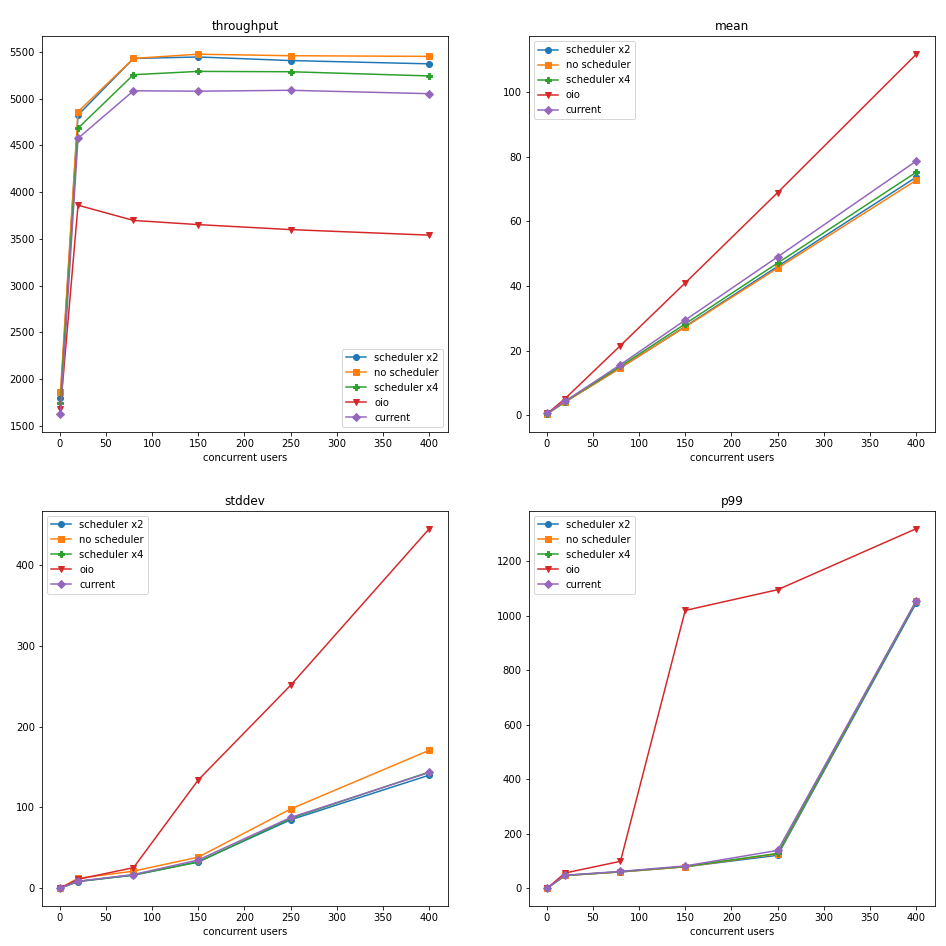
\includegraphics[scale=0.3]{figures/prime_small test results.png}
	\end{center}
	\caption{Prime test results}
	\label{prime_small_test_results}
\end{figure}


\section{Results comparison of different thread pool size}

\begin{figure}[htbp]
	\begin{center}
		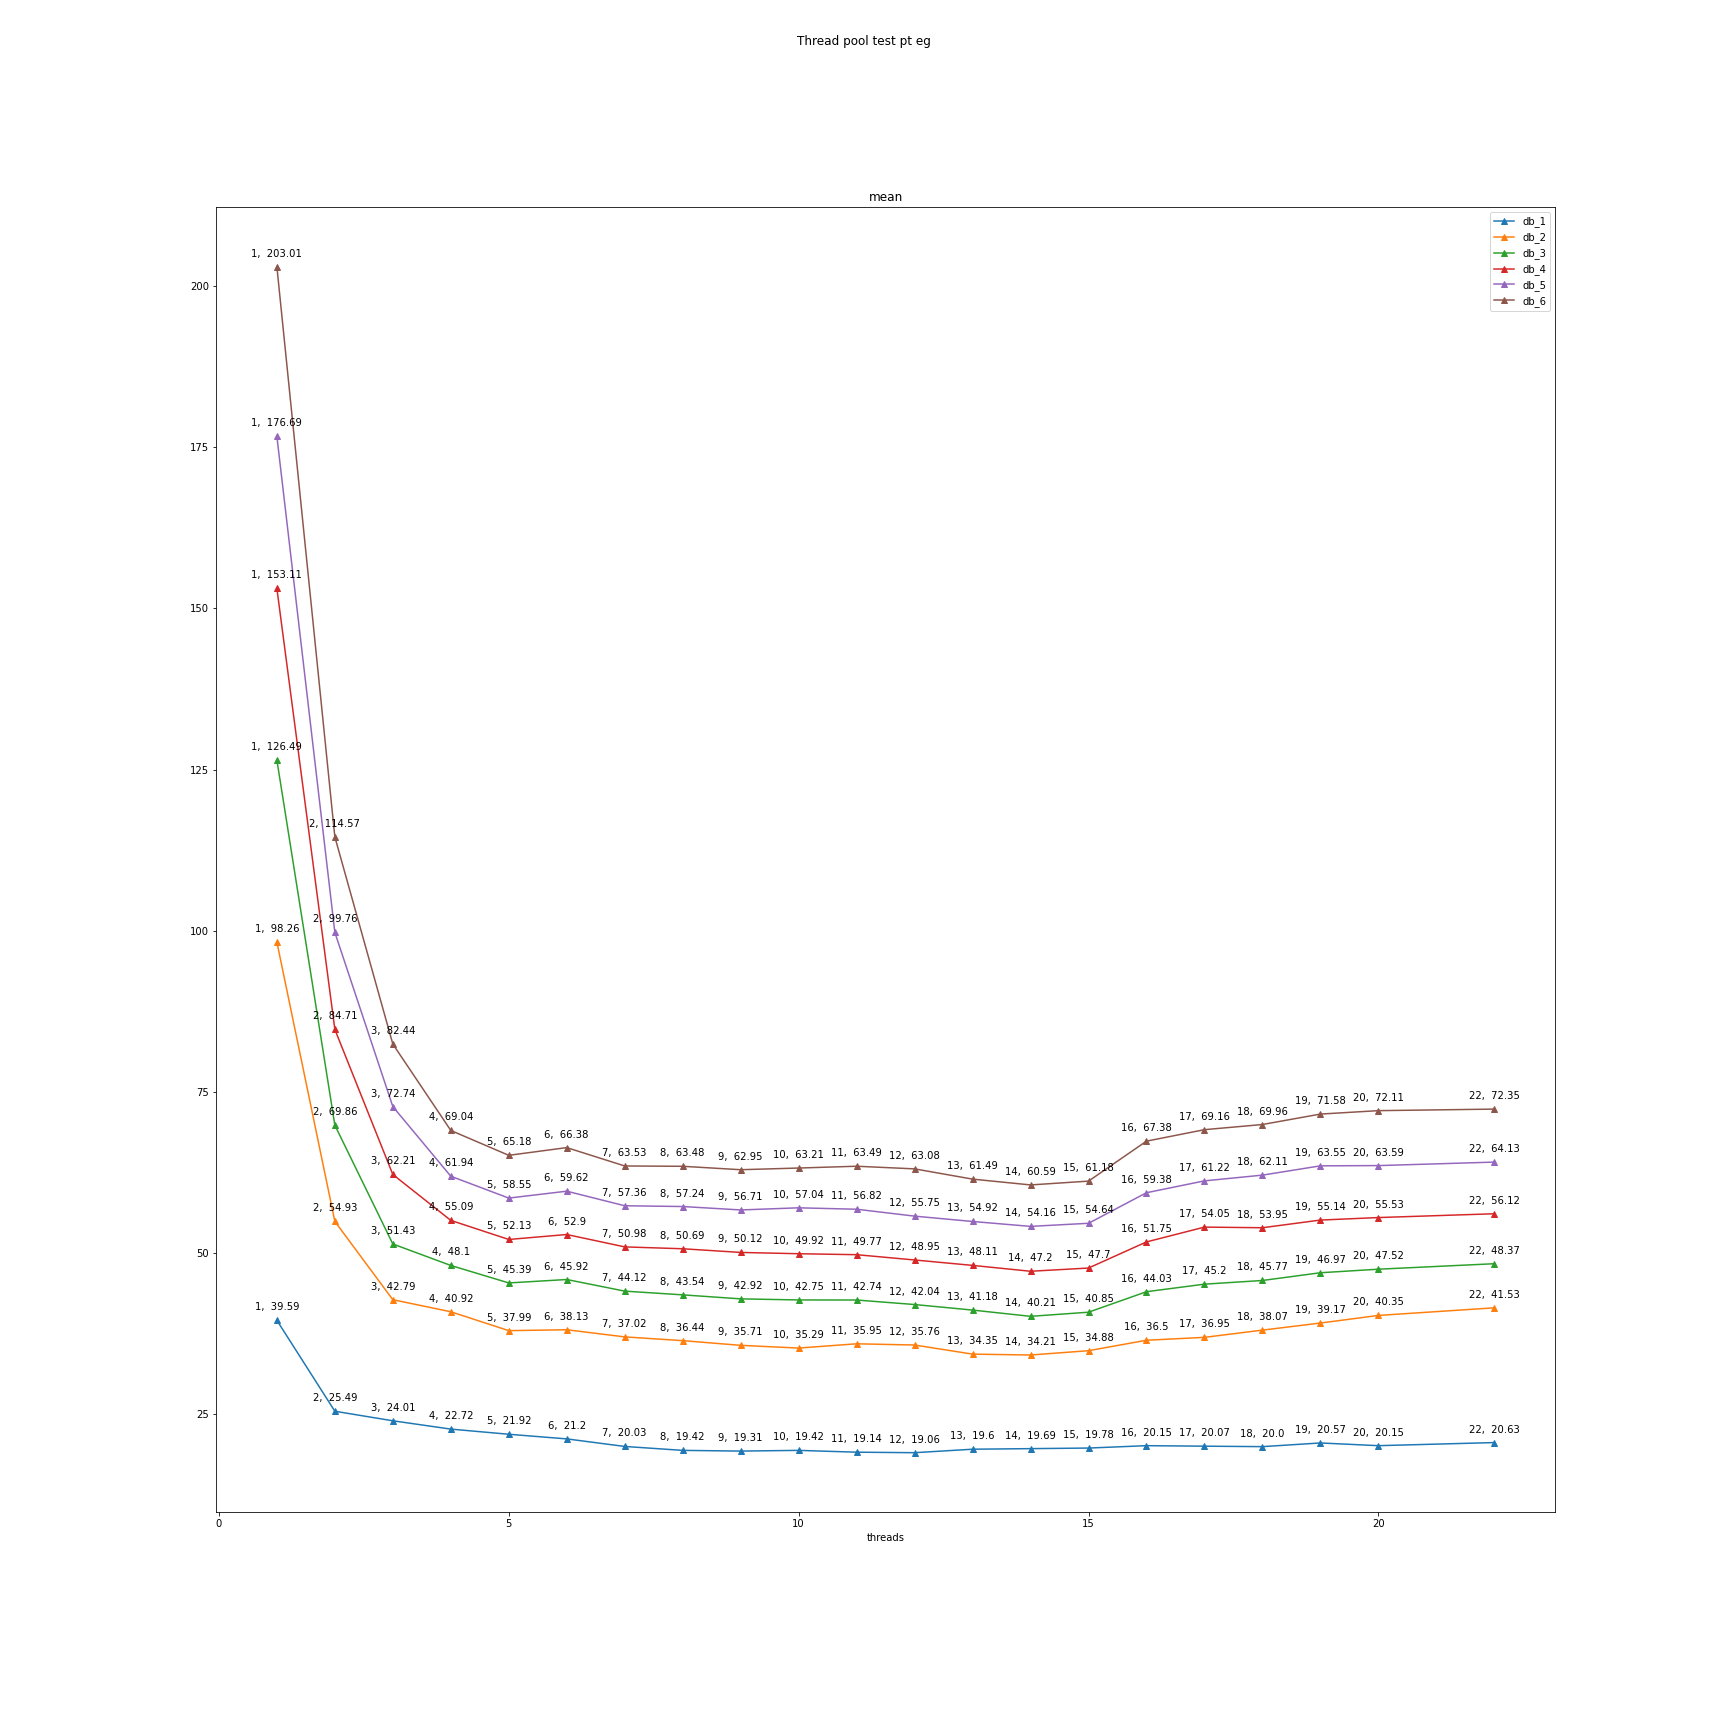
\includegraphics[scale=0.2]{figures/thread_pool_test_1.png}
	\end{center}
	\caption{Thread pool size vs Average latency}
	\label{thread_pool_test_1}
\end{figure}

\section{Results comparison of machine learning models}


\begin{figure}[htbp]
	\begin{center}
		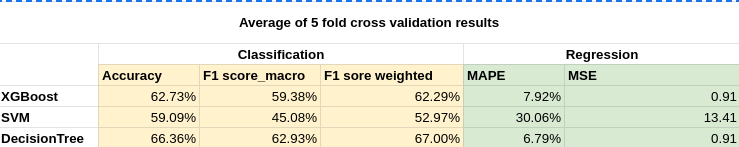
\includegraphics[scale=0.5]{figures/ml_results.png}
	\end{center}
	\caption{Results of machine learning model}
	\label{ml_results}
\end{figure}

